\begin{center}
    {\LARGE \textbf{2020有机化学，似乎不全}} \\[2ex]
    {\large 时量180分钟 \quad 满分150分}
\end{center}

\vspace{0.5cm}
\noindent\textbf{注意事项:}
\begin{enumerate}[label=\arabic*., parsep=0pt, itemsep=0pt]
    \item 答题前,考生先将自己的姓名、学号、考场号、座位号填写在答题卡上,将条形码准确粘贴在考生信息条形码粘贴区。
    \item 考试结束后,将本试卷与答题纸一并收回。
    \item 回答各个问题时,将答案写在答题纸上,写在本试卷上无效。
\end{enumerate}

\vspace{0.5cm}
\noindent\textbf{一、完成反应}

\begin{enumerate}[label=\arabic*., itemsep=3ex]
    \item 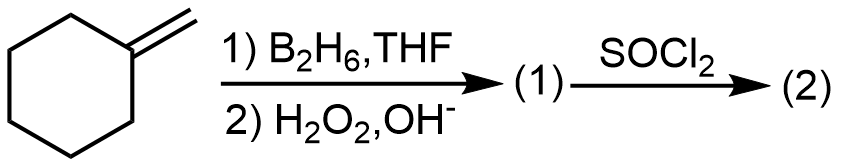
\includegraphics[scale=0.38, valign=c]{./Figure/2020/2020_1_1.png} 
    \item 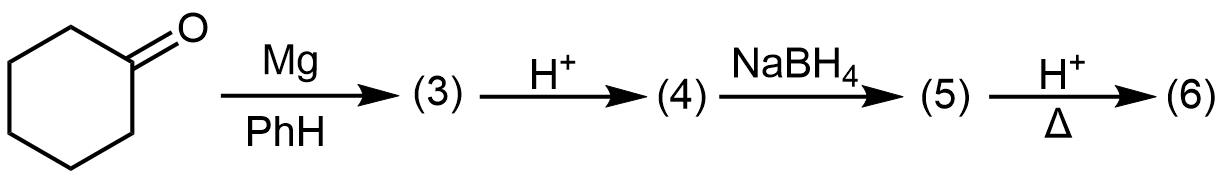
\includegraphics[scale=0.38, valign=c]{./Figure/2020/2020_1_2.png}
    \item 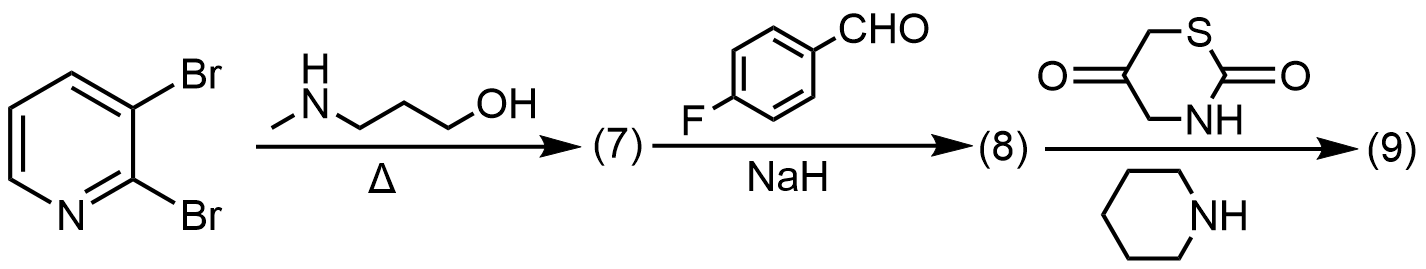
\includegraphics[scale=0.38, valign=c]{./Figure/2020/2020_1_3.png}
    \item 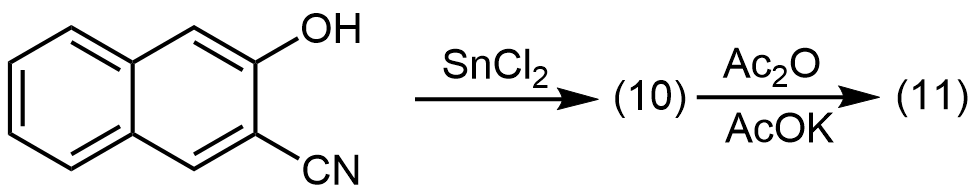
\includegraphics[scale=0.38, valign=c]{./Figure/2020/2020_1_4.png}
    \item 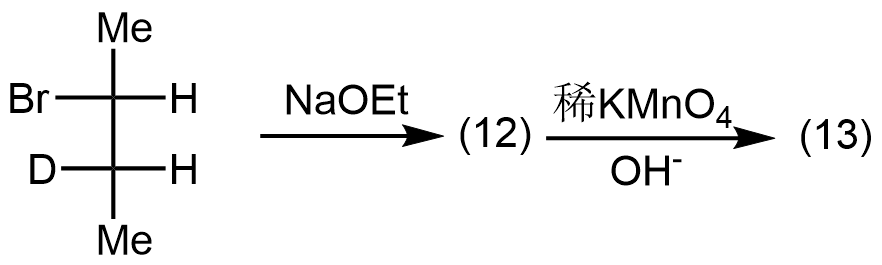
\includegraphics[scale=0.38, valign=c]{./Figure/2020/2020_1_5.png}
    \item 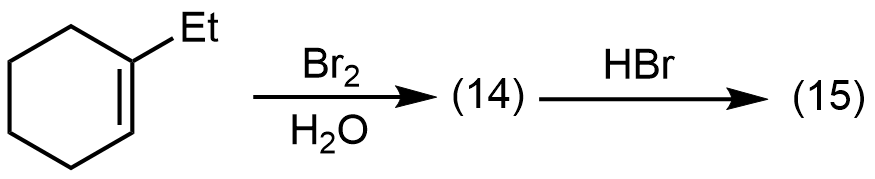
\includegraphics[scale=0.38, valign=c]{./Figure/2020/2020_1_6.png}
    \item 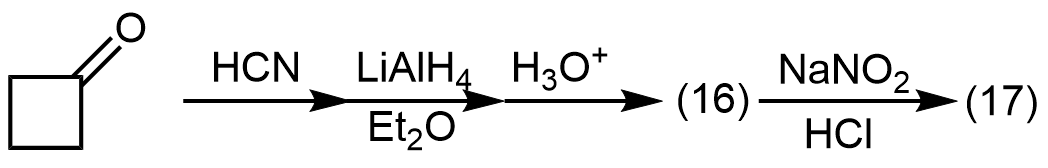
\includegraphics[scale=0.38, valign=c]{./Figure/2020/2020_1_7.png}
    \item 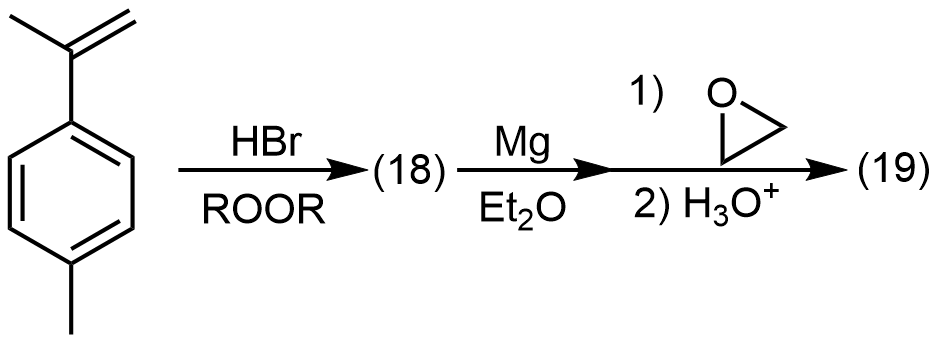
\includegraphics[scale=0.38, valign=c]{./Figure/2020/2020_1_8.png}
    \item 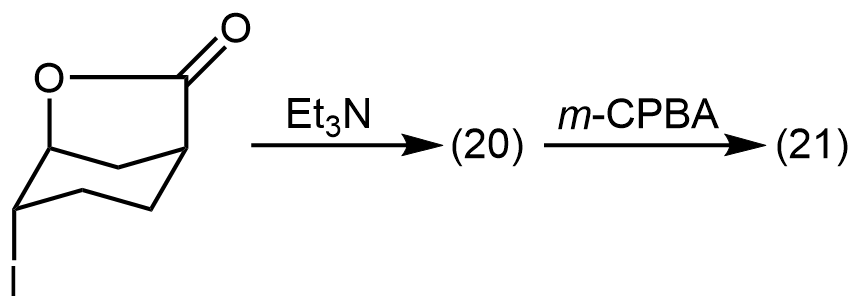
\includegraphics[scale=0.38, valign=c]{./Figure/2020/2020_1_9.png}

\end{enumerate}

\vspace{0.5cm}
\noindent\textbf{二、机理题}

\begin{enumerate}[label=\arabic*., start=1, itemsep=1.5ex]
    \item 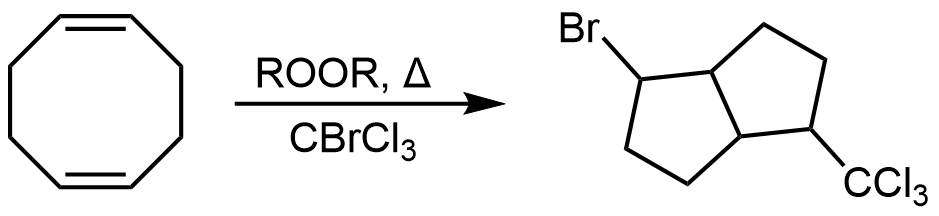
\includegraphics[scale=0.38, valign=c]{./Figure/2020/2020_2_1.png}
    \item 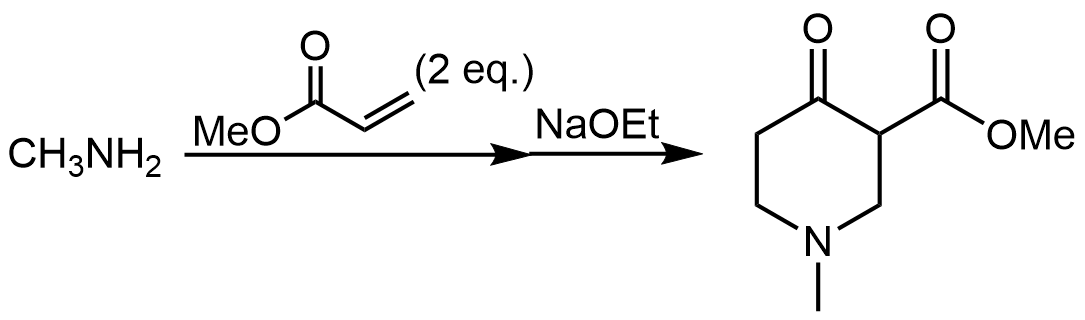
\includegraphics[scale=0.38, valign=c]{./Figure/2020/2020_2_2.png}
    \item 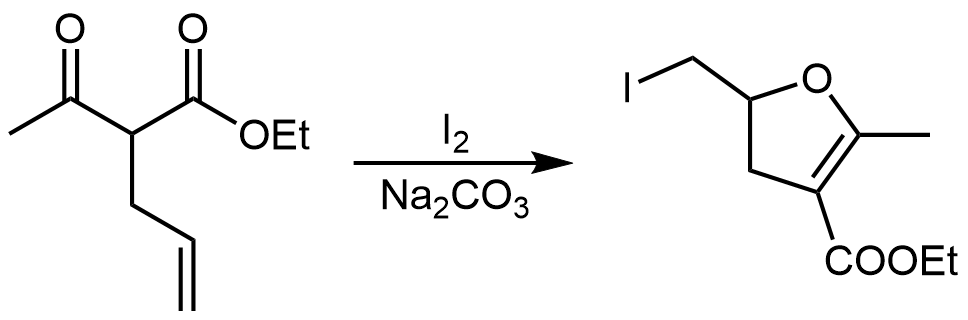
\includegraphics[scale=0.38, valign=c]{./Figure/2020/2020_2_3.png}
    \item 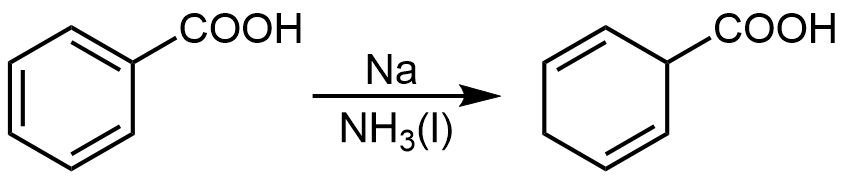
\includegraphics[scale=0.38, valign=c]{./Figure/2020/2020_2_4.png}
\end{enumerate}

\newpage

\vspace{0.5cm}
\noindent\textbf{三、合成题(42 pts.)}

\begin{enumerate}[label=\arabic*., start=1, itemsep=1.5ex]

    \begin{figure}[htbp]
        \centering
        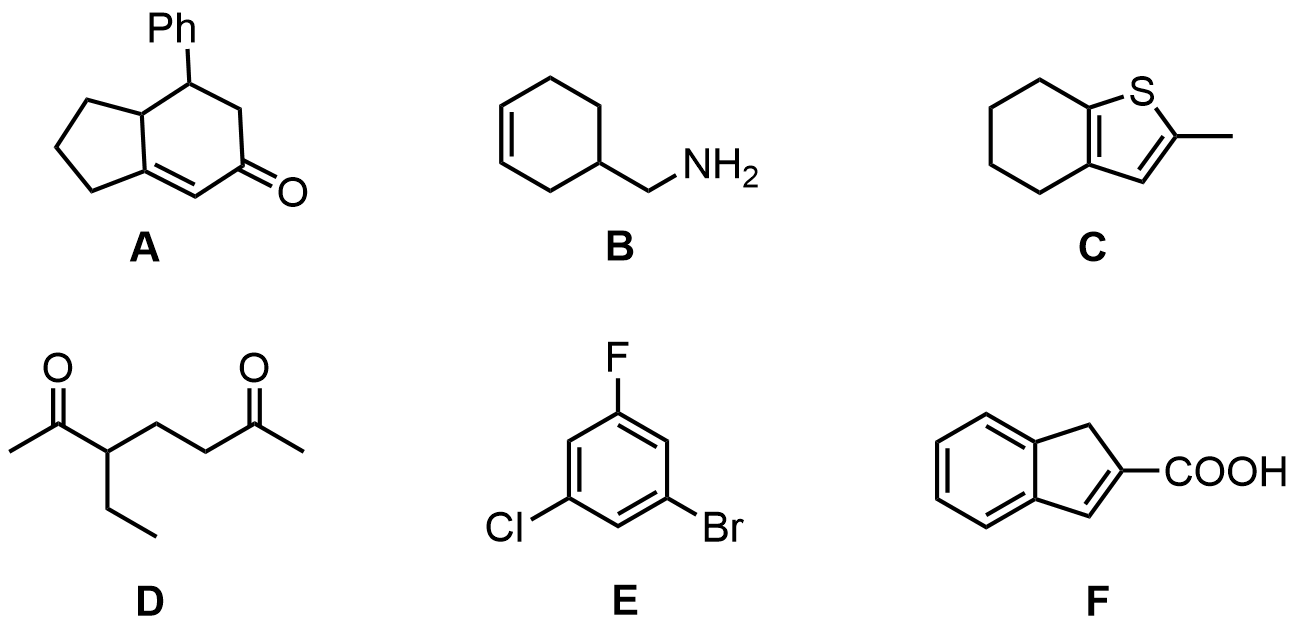
\includegraphics[scale=0.38]{./Figure/2020/2020_3.png}
    \end{figure}
    \item 以环戊酮、苯、小于等于3个碳的有机物合成\textbf{A}
    \item 以小于等于3个碳的有机物合成\textbf{B}
    \item 以环己酮、小于等于2个碳的有机物合成\textbf{C}
    \item 以乙酰乙酸乙酯、小于等于3个碳的有机物合成\textbf{D}
    \item 以苯为主要原料合成\textbf{E}
    \item 以苯、小于等于3个碳的有机物合成\textbf{F}
\end{enumerate}
